\subsubsection{Caso d'uso UC8.1.3: Creazione domanda a risposta multipla}
	\label{UC8.1.3}
	\begin{figure}[ht]
		\centering
			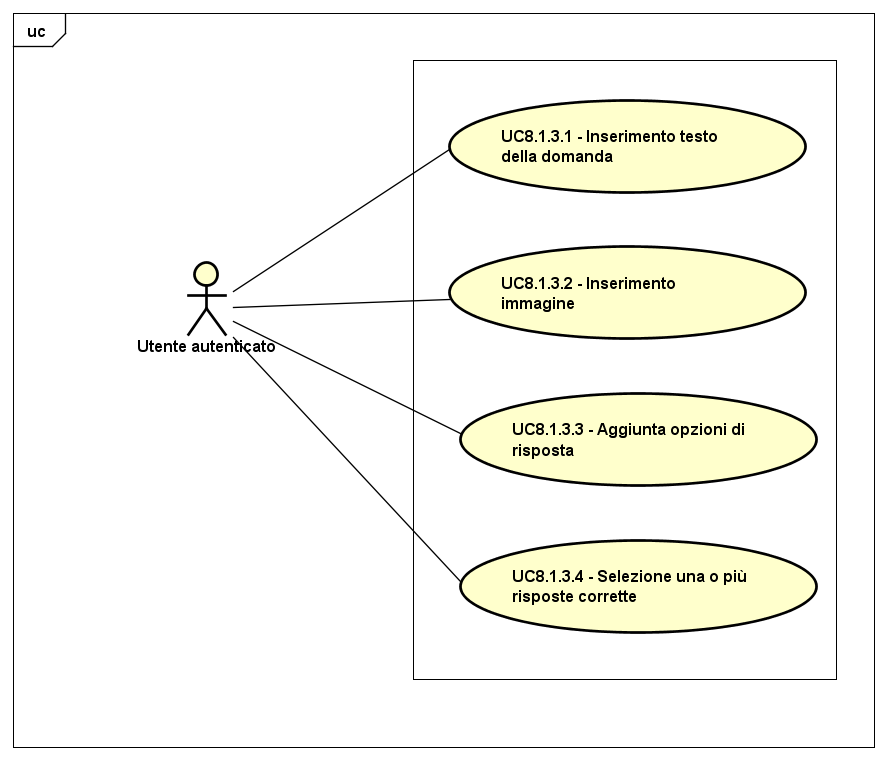
\includegraphics[scale=0.45,keepaspectratio]{UML/UC8_1_3.png}
		\caption{UC8.1.3: Creazione domanda a risposta multipla}
	\end{figure}
	\FloatBarrier
	\begin{itemize}
		\item
			\textbf{Attori}: utente autenticato, utente autenticato pro;
		\item		
			\textbf{Descrizione}: l'attore può utilizzare la procedura guidata per la creazione di una domanda a risposta multipla;
		\item
			\textbf{Precondizione}: il sistema presenta all'attore la procedura guidata per la creazione di una domanda a risposta multipla;
		\item
			\textbf{Postcondizione}: l'attore ha creato una domanda a risposta multipla;
		\item
			\textbf{Scenario principale}:
	       		\begin{enumerate}
	       			\item
	       			L'attore può inserire il testo della domanda (UC8.1.3.1);
	       			\item
	       			L'attore può inserire un'immagine relativa al testo della domanda (UC8.1.3.2);
	       			\item
	       			L'attore può aggiungere almeno due opzioni di risposta (UC8.1.3.3);
					\item
					L'attore può indicare una o più risposte corrette (UC8.1.3.4).
	 			\end{enumerate}
	\end{itemize}

\subsubsection{Caso d'uso UC8.1.3.1: Inserimento testo della domanda}
	\begin{itemize}
		\item
			\textbf{Attori}: utente autenticato, utente autenticato pro;
		\item		
			\textbf{Descrizione}: l'attore può inserire il testo della domanda;
		\item
			\textbf{Precondizione}: il sistema presenta all'attore lo spazio destinato all'inserimento del testo della domanda;
		\item
			\textbf{Postcondizione}: l'attore ha inserito il testo della domanda;
		\item
			\textbf{Scenario principale}: l'attore inserisce il testo della domanda. 
	 			
	\end{itemize}
	
\subsubsection{Caso d'uso UC8.1.3.2: Inserimento immagine}
	\begin{itemize}
		\item
			\textbf{Attori}: utente autenticato, utente autenticato pro;
		\item		
			\textbf{Descrizione}: l'attore può inserire un'immagine relativa al testo della domanda;
		\item
			\textbf{Precondizione}: il sistema presenta all'attore la funzionalità di inserimento di un immagine; 
		\item
			\textbf{Postcondizione}: l'attore ha inserito un'immagine relativa al testo della domanda;
		\item
			\textbf{Scenario principale}: l'attore inserisce l'immagine.						
	\end{itemize}


	
\subsubsection{Caso d'uso UC8.1.3.3: Aggiunta opzioni di risposta}
	\label{UC8.1.3.3}
	\begin{figure}[h]
		\centering
			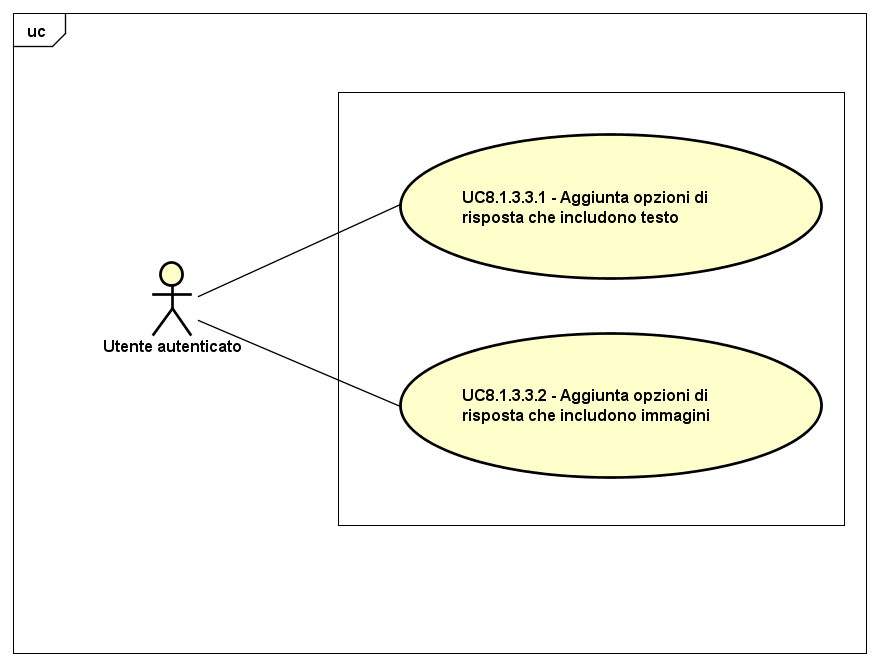
\includegraphics[scale=0.45,keepaspectratio]{UML/UC8_1_3_3.png}
		\caption{UC8.1.3.3: Aggiunta opzioni di risposta}
	\end{figure}
	\FloatBarrier
	\begin{itemize}
		\item
			\textbf{Attori}: utente autenticato, utente autenticato pro;
		\item		
			\textbf{Descrizione}: l'attore può aggiungere almeno due opzioni di risposta;
		\item
			\textbf{Precondizione}: il sistema presenta all'attore la funzionalità di aggiungere due o più opzioni di risposta; 
		\item
			\textbf{Postcondizione}: l'attore ha aggiunto due o più opzioni di risposta;
		\item
			\textbf{Scenario principale}:
	       		\begin{enumerate}
	       			\item
	       			L'attore può aggiungere opzioni di risposta che includono testo (UC8.1.3.3.1);
					\item
					L'attore può aggiungere opzioni di risposta che includono immagini (UC8.1.3.3.2).
	 			\end{enumerate}
	\end{itemize}	

\subsubsection{Caso d'uso UC8.1.3.3.1: Aggiunta opzioni di risposta che includono testo}
	\begin{itemize}
		\item
			\textbf{Attori}: utente autenticato, utente autenticato pro;
		\item		
			\textbf{Descrizione}: l'attore può aggiungere almeno due opzioni di risposta che includono testo;
		\item
			\textbf{Precondizione}: il sistema presenta all'attore la funzionalità di aggiungere due o più opzioni di risposta che includono testo;
		\item
			\textbf{Postcondizione}: l'attore ha aggiunto due o più opzioni di risposta che includono testo;
		\item
			\textbf{Scenario principale}: l'attore aggiunge due o più opzioni che includono testo.				
	\end{itemize}	

\subsubsection{Caso d'uso UC8.1.3.3.2: Aggiunta opzioni di risposta che includono immagini}
	\begin{itemize}
		\item
			\textbf{Attori}: utente autenticato, utente autenticato pro;
		\item		
			\textbf{Descrizione}: l'attore può aggiungere almeno due opzioni di risposta che includono immagini;
		\item
			\textbf{Precondizione}: il sistema presenta all'attore la funzionalità di aggiungere due o più opzioni di risposta che includono immagini;
		\item
			\textbf{Postcondizione}: l'attore ha aggiunto due o più opzioni di risposta che includono immagini;
		\item
			\textbf{Scenario principale}: l'attore aggiunge due o più opzioni che includono immagini. 				
	\end{itemize}	
		
\subsubsection{Caso d'uso UC8.1.3.4: Selezione una o più risposte corrette}
	\begin{itemize}
		\item
			\textbf{Attori}: utente autenticato, utente autenticato pro;
		\item		
			\textbf{Descrizione}: l'attore può indicare una o più risposte corrette;
		\item
			\textbf{Precondizione}: il sistema presenta all'attore la funzionalità di selezionare una o più risposte corrette;
		\item
			\textbf{Postcondizione}: l'attore ha selezionato una o più risposte corrette;
		\item
			\textbf{Scenario principale}: l'attore indica una o più risposte corrette. 			
	\end{itemize}